\documentclass[11pt,notitlepage]{article}
\makeatletter\if@twocolumn\PassOptionsToPackage{switch}{lineno}\else\fi\makeatother

%Publisher: American Association for Cancer Research
%Template Provided By: Typeset
\usepackage{booktabs}
\usepackage{amsmath,amssymb,amstext,tabulary,graphicx,times,caption,fancyhdr,float}
\usepackage[utf8]{inputenc}
\usepackage[T1]{fontenc}
\usepackage{url,lineno,microtype,subcaption}
\usepackage[onehalfspacing]{setspace}
\usepackage{wrapfig} 
\usepackage{soul}
\usepackage{caption}
\usepackage{cite}
\usepackage{algorithmic}
\usepackage{textcomp}
\usepackage{xcolor}

\usepackage{hyperref}
\hypersetup{
    colorlinks=true,
    urlcolor=blue,
    linkcolor=black,
    filecolor=black,
    citecolor=black
}


\usepackage{abstract}
\usepackage{titlesec}
\titlespacing\section{0pt}{12pt plus 4pt minus 2pt}{0pt plus 2pt minus 2pt}
\titlespacing\subsubsection{0pt}{12pt plus 4pt minus 2pt}{0pt plus 2pt minus 2pt}
\titlespacing\subsubsubsection{0pt}{12pt plus 4pt minus 2pt}{0pt plus 2pt minus 2pt}
\usepackage[paperheight=11.66in,paperwidth=8.91in,margin=1.55cm,headsep=.5cm,top=2.5cm,columnsep=.9cm]{geometry}
\renewenvironment{onecolabstract} {\vspace*{-1pc}\trivlist\item[]\leftskip\oupIndent\hrulefill\par\vskip4pt\noindent\textbf{\abstractname}\mbox{\null}\\\hspace*{.5pc}}{\par\noindent\hrulefill\endtrivlist} 
\linespread{1.13} \date{}
\captionsetup[figure]{labelfont=sc,labelfont=normal,labelsep=period,labelfont=bf,skip=1.4pt,aboveskip=1pc}
\captionsetup[table]{labelfont=sc,labelfont=bf,skip=1.4pt,labelsep=period}
\renewcommand{\headrulewidth}{0pt}
\newcommand{\diff}[2]{\frac{d #1}{d #2}}

%%%%%%%%%%%%%%%%%%%%%%%%%%%%%%%%%%%%%%%%%%%%%%%%%%%%%%%%%%%%%%%%%%%%%%%%%%
% Following additional macros are required to function some 
% functions which are not available in the class used.
%%%%%%%%%%%%%%%%%%%%%%%%%%%%%%%%%%%%%%%%%%%%%%%%%%%%%%%%%%%%%%%%%%%%%%%%%%
\usepackage{url,multirow,morefloats,floatflt,cancel,tfrupee}
\makeatletter


\AtBeginDocument{\@ifpackageloaded{textcomp}{}{\usepackage{textcomp}}}
\makeatother
\usepackage{colortbl}
\usepackage{xcolor}
\usepackage{pifont}
\usepackage[nointegrals]{wasysym}
\urlstyle{rm}
\makeatletter

%%%For Table column width calculation.
\def\mcWidth#1{\csname TY@F#1\endcsname+\tabcolsep}

%%Hacking center and right align for table
\def\cAlignHack{\rightskip\@flushglue\leftskip\@flushglue\parindent\z@\parfillskip\z@skip}
\def\rAlignHack{\rightskip\z@skip\leftskip\@flushglue \parindent\z@\parfillskip\z@skip}

%Etal definition in references
\@ifundefined{etal}{\def\etal{\textit{et~al}}}{}


%\if@twocolumn\usepackage{dblfloatfix}\fi
\usepackage{ifxetex}
\ifxetex\else\if@twocolumn\@ifpackageloaded{stfloats}{}{\usepackage{dblfloatfix}}\fi\fi

\AtBeginDocument{
\expandafter\ifx\csname eqalign\endcsname\relax
\def\eqalign#1{\null\vcenter{\def\\{\cr}\openup\jot\m@th
  \ialign{\strut$\displaystyle{##}$\hfil&$\displaystyle{{}##}$\hfil
      \crcr#1\crcr}}\,}
\fi
}

%For fixing hardfail when unicode letters appear inside table with endfloat
\AtBeginDocument{%
  \@ifpackageloaded{endfloat}%
   {\renewcommand\efloat@iwrite[1]{\immediate\expandafter\protected@write\csname efloat@post#1\endcsname{}}}{\newif\ifefloat@tables}%
}%

\def\BreakURLText#1{\@tfor\brk@tempa:=#1\do{\brk@tempa\hskip0pt}}
\let\lt=<
\let\gt=>
\def\processVert{\ifmmode|\else\textbar\fi}
\let\processvert\processVert

\@ifundefined{subparagraph}{
\def\subparagraph{\@startsection{paragraph}{5}{2\parindent}{0ex plus 0.1ex minus 0.1ex}%
{0ex}{\normalfont\small\itshape}}%
}{}

% These are now gobbled, so won't appear in the PDF.
\newcommand\role[1]{\unskip}
\newcommand\aucollab[1]{\unskip}
  
\@ifundefined{tsGraphicsScaleX}{\gdef\tsGraphicsScaleX{1}}{}
\@ifundefined{tsGraphicsScaleY}{\gdef\tsGraphicsScaleY{.9}}{}
% To automatically resize figures to fit inside the text area
\def\checkGraphicsWidth{\ifdim\Gin@nat@width>\linewidth
	\tsGraphicsScaleX\linewidth\else\Gin@nat@width\fi}

\def\checkGraphicsHeight{\ifdim\Gin@nat@height>.9\textheight
	\tsGraphicsScaleY\textheight\else\Gin@nat@height\fi}

\def\fixFloatSize#1{}%\@ifundefined{processdelayedfloats}{\setbox0=\hbox{\includegraphics{#1}}\ifnum\wd0<\columnwidth\relax\renewenvironment{figure*}{\begin{figure}}{\end{figure}}\fi}{}}
\let\ts@includegraphics\includegraphics

\def\inlinegraphic[#1]#2{{\edef\@tempa{#1}\edef\baseline@shift{\ifx\@tempa\@empty0\else#1\fi}\edef\tempZ{\the\numexpr(\numexpr(\baseline@shift*\f@size/100))}\protect\raisebox{\tempZ pt}{\ts@includegraphics{#2}}}}

%\renewcommand{\includegraphics}[1]{\ts@includegraphics[width=\checkGraphicsWidth]{#1}}
\AtBeginDocument{\def\includegraphics{\@ifnextchar[{\ts@includegraphics}{\ts@includegraphics[width=\checkGraphicsWidth,height=\checkGraphicsHeight,keepaspectratio]}}}

\DeclareMathAlphabet{\mathpzc}{OT1}{pzc}{m}{it}

\def\URL#1#2{\@ifundefined{href}{#2}{\href{#1}{#2}}}

%%For url break
\def\UrlOrds{\do\*\do\-\do\~\do\'\do\"\do\-}%
\g@addto@macro{\UrlBreaks}{\UrlOrds}



\edef\fntEncoding{\f@encoding}
\def\EUoneEnc{EU1}
\makeatother
\def\floatpagefraction{0.8} 
\def\dblfloatpagefraction{0.8}
\def\style#1#2{#2}
\def\xxxguillemotleft{\fontencoding{T1}\selectfont\guillemotleft}
\def\xxxguillemotright{\fontencoding{T1}\selectfont\guillemotright}

\newif\ifmultipleabstract\multipleabstractfalse%
\newenvironment{typesetAbstractGroup}{}{}%

%%%%%%%%%%%%%%%%%%%%%%%%%%%%%%%%%%%%%%%%%%%%%%%%%%%%%%%%%%%%%%%%%%%%%%%%%%

\newcommand{\ILF}[0]{C_\text{IL-15}}
\newcommand{\ILS}[0]{C_\text{IL-7}}
\newcommand{\MemE}[0]{M_\text{CD8}}
\newcommand{\EffE}[0]{E_\text{CD8}}
\newcommand{\MemF}[0]{M_\text{CD4}}
\newcommand{\EffF}[0]{E_\text{CD4}}
\newcommand{\norm}[1]{\|#1\|}
\newcommand{\bignorm}[1]{\bigg\|#1\bigg\|}
\newcommand{\inner}[2]{\langle #1,#2 \rangle}
\newcommand{\avg}[1]{\langle #1 \rangle}
\newcommand{\pdiff}[2]{\frac{\partial #1}{\partial #2}}
\newcommand{\ppdiff}[2]{\frac{\partial^2 #1}{\partial #2^2}}
\newcommand{\ddiff}[2]{\frac{d^2 #1}{d #2^2}}
\newcommand{\intinf}[0]{\int_{-\infty}^{\infty}}
\newcommand{\E}[0]{\mathbb E}
\newcommand{\un}[0]{u^{(n)}}
\newcommand{\vn}[0]{v^{(n)}}
\newcommand{\En}[0]{E^{(n)}}
\newcommand{\arctanh}[0]{\text{ arctanh}}



\makeatletter\def\oupIndent{1pt}
\def\author#1{\gdef\@author{\hskip-\dimexpr(\tabcolsep)\hskip\oupIndent\parbox{\dimexpr\textwidth-\oupIndent}{\centering\bfseries#1}}}
\def\title#1{\gdef\@title{\centering\bfseries\ifx\@articleType\@empty\else\@articleType\\\fi#1}}
\let\@articleType\@empty \def\articletype#1{\gdef\@articleType{{\normalfont\itshape#1}}}

\AtBeginDocument{\fancypagestyle{plain}{\renewcommand{\headrulewidth}{0pt}\renewcommand{\footrulewidth}{0pt}\fancyhf{}}}
\makeatother


%\title{Mathematical Modeling of Cell Cycle Dynamics and Whole-Genome Doubling in Response to Gemcitabine Treatment}
\title{Mathematical modeling of gemcitabine sensitivity as a function of ploidy}
\author{Authors: XX}

\begin{document}

\maketitle

\section*{Abstract}
Aneuploidy is a hallmark of cancer. Thereby, there have been ongoing efforts investigating the potential of ploidy as a predictive biomarker for therapy response in cancer. However, no therapeutic agent has been yet approved as synthetically lethal with aneuploidy. In this study, we identify that near-diploid triple-negative breast cancer (TNBC) cells are hypersensitive to gemcitabine treatments. In contrary, near-tetraploid TNBC cells could grow into polyaneuploid giant cancer cells (PACCs) thru whole genome doubling (WGD) and continue to safely grow in the presence of gemcitabine. Such cells adopted an endoreplication in which the genome replicates, mitosis is omitted, and cells grow in size. These PACCs re-entered the proliferative cell cycle and grew in cell number when treatment was terminated. Altogether, PACC formation and WGD represent a fundamental cellular response to gemcitabine, and contributes to therapy resistance or tumor relapse in a ploidy-dependent manner in TNBCs. Moreover, to facilitate the translation of ploidy as a biomarker into clinical practice, any such individualization of medical interventions requires a deep understanding, complex evaluation and integration of tumor characteristics at a variety of levels including the disciplines of genetics, cell biology, biochemistry, pharmacology and chemical biology. Therefore, we created a novel three-tier framework including in-silico, computational and experimental components, which not only predicts gemcitabine response based on ploidy status, but also mathematically calculates the optimal dosage for individual treatments.
\section*{Introduction}

Polyploid/ polyaneuploid giant cancer (PGCC/PACC) (PACC henceforth) state is a common response of cancer cells to various stressors including chemotherapy, irradiation, hypoxia and viral infection. Upon stress, PACCs adopt an endoreplication in which the genome replicates, mitosis is omitted, and cells grow in size, leading to resistance. How accessible WGD is to a cell, therefore, directly translates to its resistance to therapy. In this study, we hypothesized that WGD and PACC state are more plausible to cancer cells that already have a higher ploidy content prior to therapy. To test this hypothesis, we developed a comprehensive three-tier framework consisting of i) computational, ii) in vitro and iii) in silico components.
We designed a set of ordinary differential equations (ODEs) to model how cells enter and exit the PACC state in response to a given stressor. We engineered how this in silico approach interacts with in vitro experiments into a broadly applicable software solution called CLONEID. The software uses computer vision to monitor phenotypic changes in cell and nuclear size from standard bright-field microscopy and classify cells into PACC and non-PACC states. We used CLONEID to test various therapeutic agents for their ability to select for a stable near-tetraploid population in a set of near-diploid cell lines. Through spontaneous cell fusions, we also obtained tetraploid breast cancer cells matched with their parental lines. Altogether, this framework, now, enables us to monitor the PACC state experimentally in matched cell lines with differential DNA content to model the successful entrance and exit rates to and from the endoreplication state, respectively.
As the first application of this framework, we tested the ability of our matched triple-negative breast cancer (TNBC) lines to access the PACC state upon treatment with 18 commonly-used chemotherapy agents. We observed that gemcitabine caused continued cell growth without cell division in both tetraploid SUM-159 and MDA-MB-231 cells whereas near-diploid parental cells were hypersensitive to the treatment. Consequently, tetraploid cancer cells continued to safely grow in the presence of gemcitabine. Furthermore, these PACCs re-entered the proliferative cell cycle and grew in cell number when treatment is terminated.
\clearpage
\section*{Methods}
% \subsubsection*{Model 1}

% Hypothesis 1: 
% Cells continue to divide under treatment, but most of them die in the process. Over time resistance develops as dividing cells reduce their apoptotic risk.\newline


% We use a log-kill pattern for modeling treatment effect, which assumes that the shrinkage rate of the population as a result of drug treatment is proportional to population size:


% \begin{equation} \label{m1}
% \frac{\mathrm{d} T}{\mathrm{~d} t}=f(T)-k_{\mathrm{d}} \cdot e^{-\lambda \cdot t} \cdot \text { Exposure } \cdot T
% \end{equation}

% The $e_{-\lambda \cdot t}$ term quantifies the decline of drug effect over time (i.e. resistance) and $f(T)$ is the growth term. For example, for logistic growth we have: $f(T) = r \cdot T \cdot (1 - \frac{T}{K})$

\subsection*{Cell viability and cell death assay}
Cell viability assays were carried out using the IncuCyte live-cell imaging system (Sartorius). Briefly, 2N and 4N SUM-159-NLS-mCherry cells were plated in four replicates in 96-well plates (Falcon, Corning, New York, USA) at a density of 1000 cells per well and treated with a 10-point 2X serial dilutions of gemcitabine within the concentration range of 0 and 800 nM. Sytox Deep Red (S11381, ThermoFisher Scientific) nucleic acid stain was also added to monitor dead cells. Plates were then incubated in the IncuCyte CO2 incubator for 10 days while four separate images were captured from each well every 2 hours using 10× objective in red, infrared and phase channels. Red object count (ROC) per well was calculated as a measure of viable cells and near-infrared object counts (NOC) per well was calculated as a measure of dead cells when the treatment was performed.

\subsection*{PKPD measurement of intracellular dFdCTP}
To construct the intracellular drug-action input for the live/dead model, we used PKPD measurements of gemcitabine metabolites collected for the matched 2N and 4N cell states. The live/dead model was driven by the intracellular active metabolite dFdCTP, rather than by parent gemcitabine concentration. For each ploidy, PKPD sheets corresponding to the main-dose and low-initial-dose gemcitabine conditions were used to define calibrated dFdCTP time courses. The main 2N and 4N PKPD sheets were treated as \(1.0~\mu\mathrm{M}\) gemcitabine reference-dose profiles, whereas the low-initial-gemcitabine 2N and 4N sheets were treated as \(0.1~\mu\mathrm{M}\) reference-dose profiles.

PKPD dFdCTP measurements were reported in ng/mL and converted to \(\mu\mathrm{M}\)-equivalent concentrations using the dFdCTP molecular weight,
\[
503.1~\mathrm{ng}/\mathrm{nmol}.
\]
Because
\[
1~\mathrm{nmol}/\mathrm{mL}=1~\mu\mathrm{M},
\]
the conversion was
\[
C_{\mathrm{dFdCTP}}~(\mu\mathrm{M})
=
\frac{C_{\mathrm{dFdCTP}}~(\mathrm{ng}/\mathrm{mL})}
{503.1~\mathrm{ng}/\mathrm{nmol}}.
\]
The resulting dFdCTP profiles were baseline-subtracted using the first measured time point so that the model input represented treatment-induced intracellular dFdCTP above the initial measured level.

\subsection*{Image analysis}
 \subsubsection*{Cell segmentation and classification with HALO}

Cell segmentation was achieved by training a single-cell segmentation neural network in Halo-AI platform [1]. At the beginning, a training dataset was collected by selecting a subsample of images from the data. Two main selection criteria were considered during the image sampling. First, the training set must have representative images from both 2N and 4N cells. Second, multiple images were sampled from different time points for each cell type 2N and 4N to ensure the capture of cell change over time during the training process. After the selection of train set, nucleus of cells was labeled using Halo built-in labeling tools. Finally, the training process was performed until all cells are accurately segmented. 
Another object classifier was trained on the top of the cell segmentation classifier results to classify each segmented cell to either dead, alive or transitional cell. At the beginning, cells are labeled either dead or alive by tracking the cells over the time and by observing changes in their nuclei. The object classifier was trained iteratively until the cell were classified correctly.

[1] HALO Image Analysis Platform version 3.6.4134 and HALO AI version 3.6.4134 (Indica Labs, Inc.), Albuquerque, NM: Indica Labs, Inc.; 2023.

\subsubsection*{Tracking live cells with Ilastik}

Initially, all images and their classified cell masks were compiled and put together into time series and saved as tiff files. Each time series consists of a set of images/timepoints that were put in a natural temporal ordering. Subsequently, to minimize the error in cell tracking, the timepoints in each time series were sequentially co-registered by aligning each timepoint to the timepoint before it. Rigid cross correlation registration algorithm in [2] was used to align timepoints.

Lastly, Ilastik (ver 1.4.0) was used to train a structured learning cell tracking pipeline [3]. The pipeline was trained by giving the algorithm some examples of cell trajectories/lineages over time. The training examples were selected to cover all possible scenarios of cell changes such as division, dying, or merging over the course of time. The given examples were used to optimize for the weights associated with cell detections, transitions, divisions, appearances, and disappearances [4].  Moreover, other tracking parameters were adjusted to impose more restrictions on the tracking process. An example of the restrictions is applying a penalty on the appearance of new cells that weren’t a result of cell division (in some cases, cells clump together on one frame, and then they split in the next frame, then clump again the subsequent frame).  The values of the tracking parameters were selected by running the tracking several times with different values and select the parameter value that provided the best tracking results.

[2] Manuel Guizar-Sicairos, Samuel T. Thurman, and James R. Fienup, "Efficient subpixel image registration algorithms," Opt. Lett. 33, 156-158 (2008).

[3] Berg, S., Kutra, D., Kroeger, T. et al. ilastik: interactive machine learning for (bio)image analysis. Nat Methods 16, 1226–1232 (2019). https://doi.org/10.1038/s41592-019-0582-9

[4] M. Schiegg, P. Hanslovsky, B. X. Kausler, L. Hufnagel, F. A. Hamprecht. Conservation Tracking. Proceedings of the IEEE International Conference on Computer Vision (ICCV 2013), 2013.

\subsubsection*{Track classification}

Let $x_t$ be a parental cell at the last timepoint $t$ before its cell division event gives rise to two daughter cells $a_{t+1}$ and $b_{t+1}$. We further refer to all such parental and daughter cells as pre- and post-division tracks respectively. Further we refer to all post-division tracks for which there exists a timepoint $\tau > t+1$ at which they give rise to two daughter cells, as inter-division tracks between timepoints $t+1$ and $\tau - 1$.

We identified xx inter-division tracks in untreated wells which lasted at least 18 hours (doubling time for SUM-159 is 22 hours). For XX (XX\%) of these we observed a strong correlation between time and cell area (Pearson r>=xx), suggesting these are indeed cells that progress through the cell cycle.
XX: we manually validated XX of these tracks, using the tracking accuracy measure (TRA, see http://celltrackingchallenge.net/evaluation-methodology). Validation confirmed the correctness of these tracks as well as antecedent and subsequent cell division events (accuracy = XX).\newline

We excluded low-quality tracks based on these criteria: (i) Daughter-parent cell intervals of less than 18 hours, (ii) Cell death fraction \( > 10\% \), (iii) Weak correlation between cell size and time (Pearson \( r < 0.3 \)).


\section*{Results}


\subsection*{A dFdCTP-driven delay model captures gemcitabine live/dead dynamics across ploidy states}

We first asked whether time-resolved live/dead imaging data could be explained by a compact model in which gemcitabine response is driven by intracellular dFdCTP exposure, rather than by the administered extracellular gemcitabine dose alone. To this end, we fit a joint alive/dead count model across gemcitabine doses, replicates, and ploidy states. The default model used an intracellular dFdCTP signal surface derived from the PKPD measurements, an empirical dose-response correction consisting of a ploidy-specific power-law term and a shared Hill gate, immediate cytostasis, delayed cytotoxicity through a transit chain, and drug-independent baseline and confluence-associated death.

The fitted model reproduced the major features of the live and dead object trajectories across both 2N and 4N cells (Fig.~\ref{fig:default_gem_live_dead_fit}). In particular, the model captured the high-dose decline in live cells, the delayed accumulation of dead objects, and the qualitative separation between low-dose, intermediate-dose, and high-dose gemcitabine responses. The best fit was obtained with \(n_{\mathrm{tr}}=5\) transit compartments, with posterior objective \(61{,}603.75\), data negative log likelihood \(61{,}597.53\), and prior penalty \(6.22\) across 8,780 alive/dead observations (Table~\ref{tab:gem_best_fit_parameters}; Supplementary Table~\ref{tab:ntr_model_comparison}). The negative-binomial dispersion parameters were \(\theta_A=6.95\) for alive counts and \(\theta_D=7.76\) for dead counts, consistent with substantial but finite overdispersion in both imaging channels.


\begin{table}[htbp]
\centering
\caption{Best-fit parameters for the default gemcitabine live/dead model.}
\label{tab:gem_best_fit_parameters}
\begin{tabular}{lcc}
\toprule
Parameter & 2N & 4N \\
\midrule
\(r\) (day\(^{-1}\)) & 1.25 & 1.78 \\
\(K\) & 25,358 & 20,512 \\
\color{blue} \(k_{\mathrm{tr}}\) (day\(^{-1}\)) & 6.84 & 2.82 \\
\color{blue} \(n_{\mathrm{tr}}\) (chains) & 5 & 5 \\
\(k_{\mathrm{kill}}\) & 217.3 & 129.9 \\
\(k_{\mathrm{clear}}\) (day\(^{-1}\)) & 0.152 & 0.062 \\
\(k_{\mathrm{cyto}}\) & 8041 & 1163 \\
\(\beta\) & 0.253 & 0.488 \\
\(\mu_{\mathrm{base}}\) (day\(^{-1}\)) & 0.117 & 0.017 \\
\(\mu_{\mathrm{conf}}\) (day\(^{-1}\)) & 0.051 & 0.054 \\
\bottomrule
\label{bestfitparams}
\end{tabular}
\end{table}


 \begin{figure}
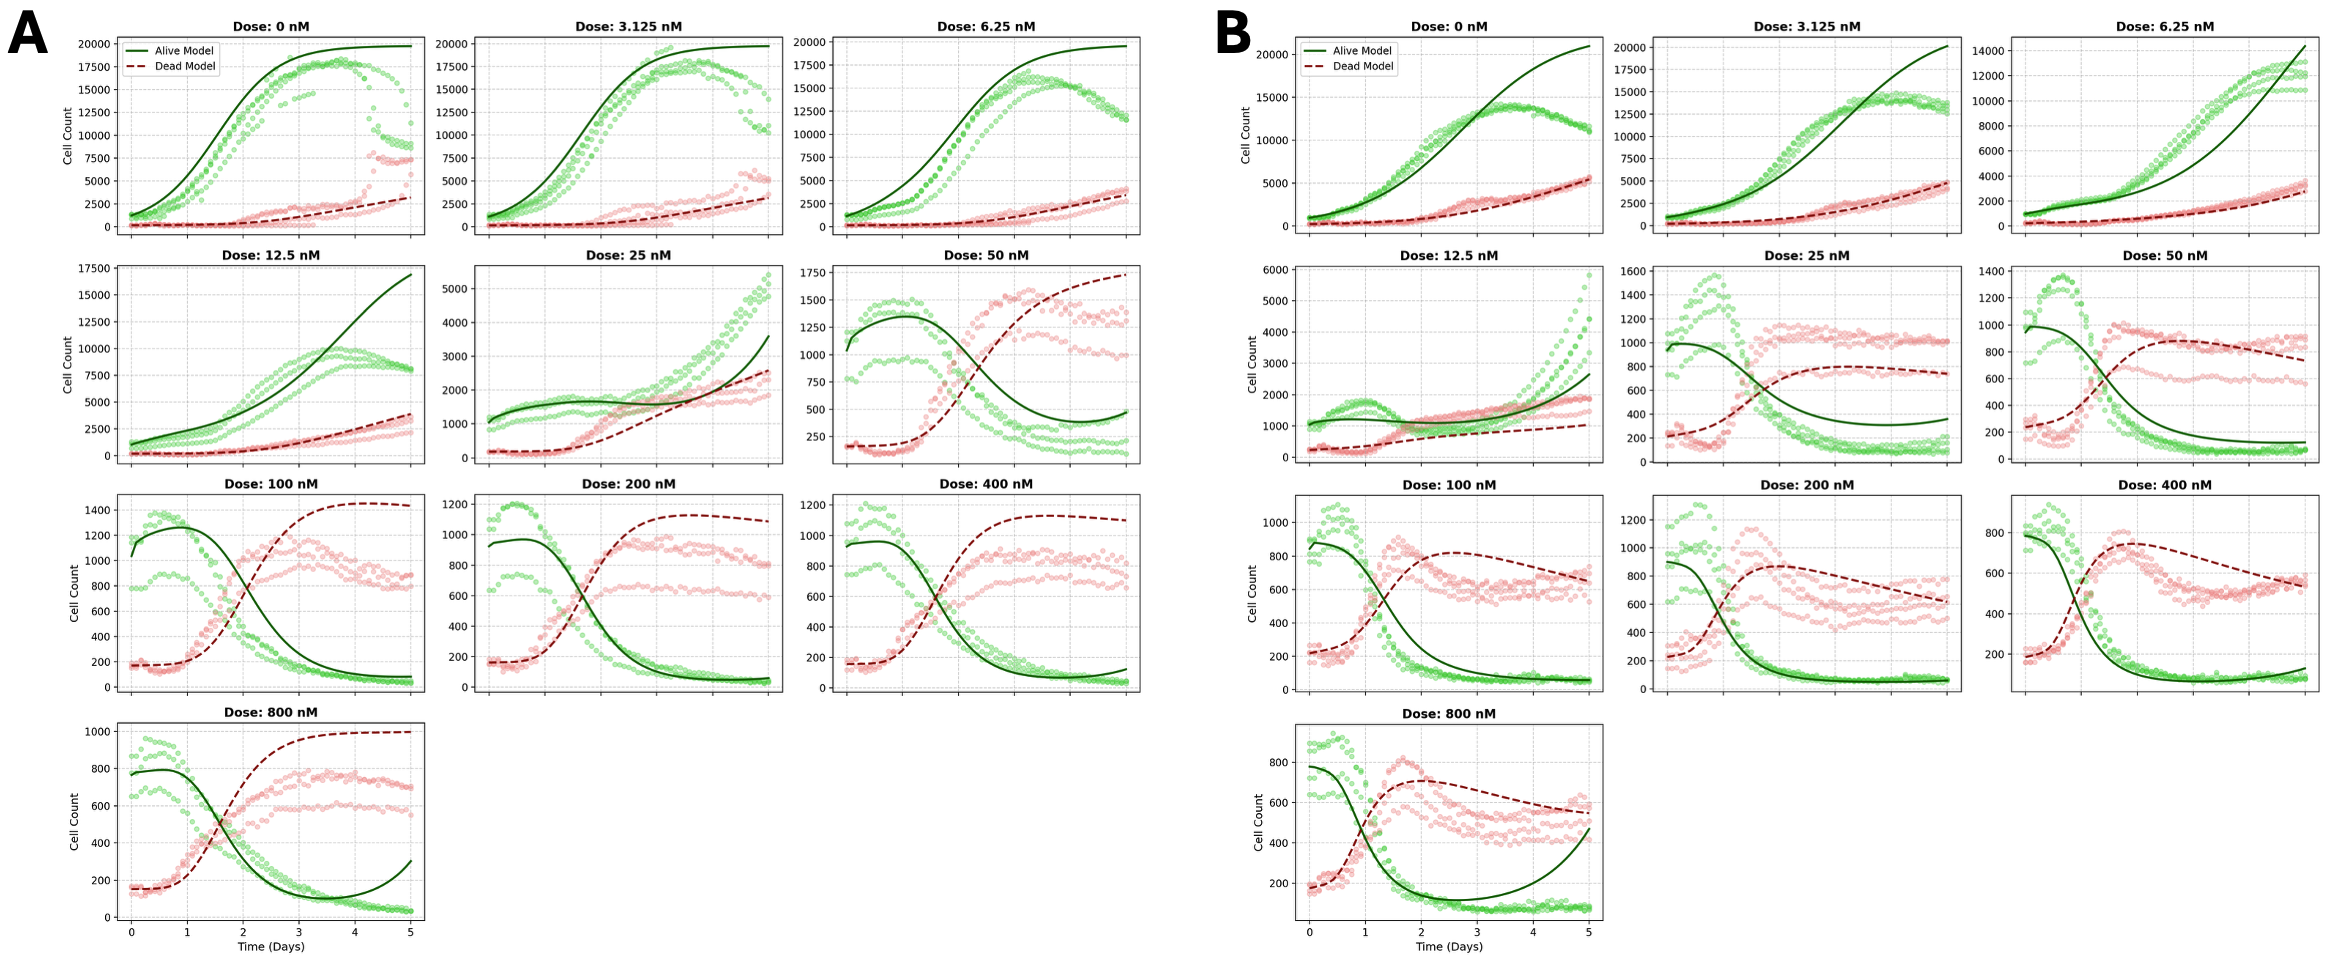
\includegraphics{Figs/invitrojointfits.png}
\caption{\textbf{Cohort-level joint fits of the default gemcitabine live/dead model for 2N
  and 4N cells.}
  (A) 2N cohort fit. (B) 4N cohort fit. In each dose panel, points show observed alive and
  dead object counts over time across replicate wells, and the solid/dashed curves show the
  corresponding model-predicted alive and dead trajectories from the best cohort-level fit.
  The fitted model was the intracellular dFdCTP-driven Model, with immediate
  cytostasis, delayed drug-induced death, ploidy-specific $\beta$ dose correction, a fitted
  shared Hill dose gate, baseline death, and fitted confluence-associated death. Parameters
  were inferred jointly across doses within each ploidy using the alive/dead negative-binomial
  objective. Control ($0$ nM) trajectories are included to show baseline growth and death
  behavior in the absence of treatment.}
\label{default_gem_live_dead_fit}
\end{figure}



\subsection*{Gemcitabine-induced death is delayed, with longer inferred delay in 4N cells}

The transit-chain component provided an empirical estimate of the delay between effective intracellular dFdCTP exposure and observed death. For the best model, \(n_{\mathrm{tr}}=5\). The fitted transit rates were \(k_{\mathrm{tr},2N}=6.84~\mathrm{day}^{-1}\) and \(k_{\mathrm{tr},4N}=2.82~\mathrm{day}^{-1}\), corresponding to approximate mean delays \(n_{\mathrm{tr}}/k_{\mathrm{tr}}\) of 0.73 days (\(\sim 17.5\) hours) for 2N cells and 1.77 days (\(\sim 42.5\) hours) for 4N cells. Thus, although the model does not explicitly track cell-cycle states, it infers a substantially longer delay from effective gemcitabine activity to death commitment in 4N cells.

The fitted potency parameters also differed by ploidy. The 2N cells had higher fitted drug-induced cytotoxic potency (\(k_{\mathrm{kill},2N}=217.3\)) than 4N cells (\(k_{\mathrm{kill},4N}=129.9\)). Similarly, immediate cytostatic potency was larger in 2N cells (\(k_{\mathrm{cyto},2N}=8041\)) than in 4N cells (\(k_{\mathrm{cyto},4N}=1163\)). Together, these results indicate that the fitted model attributes the stronger gemcitabine sensitivity of 2N cells to both stronger immediate proliferation suppression and stronger delayed death, whereas 4N cells exhibit a slower delayed-death timescale (Fig.~\ref{fig:ploidy_parameter_fold_change}; Table~\ref{tab:gem_best_fit_parameters}).

\begin{figure}[htbp]
    \centering
    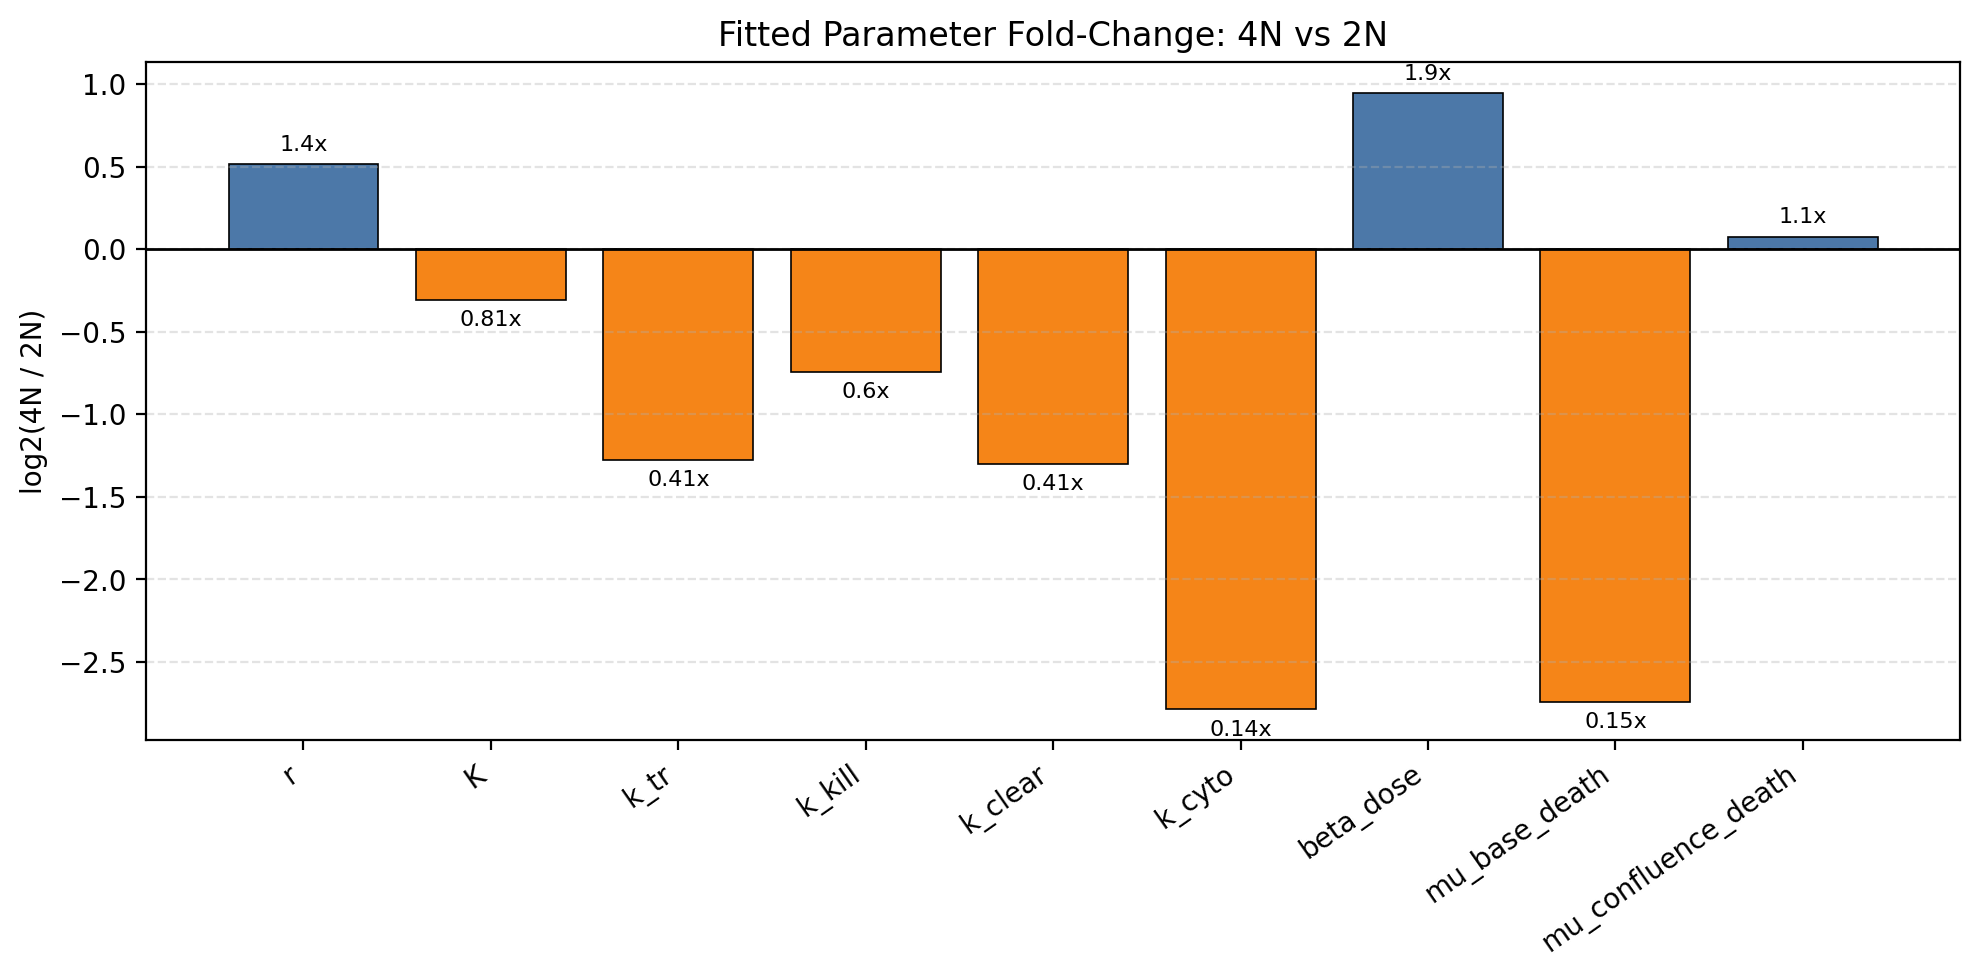
\includegraphics[width=0.8\textwidth]{Figs/ploidy_parameter_log2_fold_change.png}
    \caption{
    Ploidy-associated parameter differences in the default gemcitabine model. Bars show log$_2$ fold-changes comparing 4N to 2N fitted parameter values. Negative values indicate lower fitted values in 4N cells. The 4N fit shows a lower transit rate, corresponding to a longer inferred delay from effective dFdCTP exposure to death commitment.
    }
    \label{fig:ploidy_parameter_fold_change}
\end{figure}

\subsection*{The fitted dose-response correction identifies a low-dose activation threshold}

The initial PK-derived dFdCTP signal surface was insufficient by itself to align the lowest and intermediate gemcitabine doses. The best model therefore included a fitted effective dose-response correction consisting of a ploidy-specific power-law term and a shared Hill gate. The fitted Hill gate had \(EC_{50}=0.0185~\mu\mathrm{M}\), corresponding to approximately 18.5 nM, and Hill coefficient \(h=2.69\). This placed the inferred activation threshold in the dose range where the live/dead trajectories transition from near-control behavior to substantial response.

The combined correction factor was strongly dose-dependent (Table~\ref{tab:effective_dose_scaling}). For 2N cells, the correction suppressed the lowest doses relative to the 100 nM reference, with combined correction factors of 0.111 at 3.125 nM and 0.408 at 6.25 nM, while boosting the intermediate-low dose range, with correction factors of 1.229 at 12.5 nM, 1.967 at 25 nM, and 1.586 at 50 nM. The corresponding 4N correction factors were 0.049, 0.213, 0.755, 1.421, and 1.348. Thus, the fitted dose mapping imposed little effective drug action at the lowest doses, amplified the intermediate response range, and compressed higher doses relative to the reference.

This fitted dose correction is empirical and should not be interpreted as a direct measurement of dFdCTP biochemistry. Rather, it represents the effective mapping from administered gemcitabine dose and PK-derived intracellular dFdCTP signal to the live/dead response observed in this assay.

\subsection*{The in vitro model provides a ploidy-dependent delay kernel for downstream in vivo modeling}

The fitted in vitro model provides two distinct kinds of information: a temporal delay kernel linking effective gemcitabine activity to observed death, and assay-specific potency parameters controlling the magnitude of cytostasis and death. For downstream in vivo modeling, we use the delay kernel as the more transferable component (see Methods XX).


  
\clearpage

\renewcommand{\figurename}{Supplementary Figure}
\setcounter{figure}{0}  
\renewcommand{\tablename}{Supplementary Table}
\setcounter{table}{0}  



\section*{Supplementary Information}


\subsection*{In-vitro Delay-aware cytostasis and cytotoxicity model for gemcitabine}


\paragraph{Intracellular dFdCTP signal surface.}
The default in vitro gemcitabine live/dead model is driven directly by a ploidy-specific intracellular dFdCTP signal surface rather than by parent extracellular gemcitabine pharmacokinetics. For ploidy $p\in\{2N,4N\}$, administered gemcitabine dose $d$ (in $\mu$M), and time $t$ (in days), the PK-derived intracellular signal is denoted
\[
C_{\mathrm{dFdCTP},p}^{\mathrm{PK}}(t,d).
\]
This signal surface is built from the \texttt{dFdCTP (ng/mL)} PKPD measurements after conversion to $\mu$M-equivalent units and subtraction of the baseline ($t=0$) signal for each calibrated PK sheet. Each calibrated dose retained its own measured time course. Terminal behavior was represented by a fitted exponential tail when the post-peak decay phase was identifiable; otherwise, a predefined fallback half-life of 1 day was used for that dFdCTP profile. Within the calibrated dose range, the surface interpolates dFdCTP values across dose in log-dose space. Below the minimum calibrated PK dose, the temporal profile at the minimum calibrated dose is preserved and scaled proportionally with dose. At zero administered dose, the intracellular dFdCTP signal is defined to be zero.

\paragraph{Effective dose-response correction.}
For the default fits reported here, we used the beta--Hill baseline/confluence-death model. The effective intracellular dFdCTP signal combines a ploidy-specific power-law dose correction with a shared normalized Hill dose gate,
\[
\widetilde{C}_{p}(t,d)
=
C_{\mathrm{dFdCTP},p}^{\mathrm{PK}}(t,d)
\left(\frac{d}{d_{\mathrm{ref},p}}\right)^{\beta_p-1}
G(d;EC_{50},h,d_{\mathrm{ref},p}),
\]
where $d_{\mathrm{ref},p}$ is the minimum calibrated PK reference dose for ploidy $p$ and $\beta_p$ is a ploidy-specific dose-scaling exponent. This choice preserves the PK-derived signal when $\beta_p=1$ and allows sublinear or supralinear effective dose scaling when $\beta_p\neq 1$. The shared Hill gate is
\[
G(d;EC_{50},h,d_{\mathrm{ref},p})
=
\frac{H(d;EC_{50},h)}{H(d_{\mathrm{ref},p};EC_{50},h)},
\qquad
H(d;EC_{50},h)=\frac{d^h}{EC_{50}^h+d^h},
\]
where $EC_{50}$ and $h$ are shared fit parameters. At $d=0$, the effective signal is set to $\widetilde{C}_p(t,0)=0$.

\paragraph{Immediate cytostasis and distributed delay to death.}
Drug-induced proliferation suppression is driven by the \emph{immediate} effective dFdCTP signal. The cytostatic multiplier is
\[
m_{\mathrm{cyto},p}(t,d)
=
\frac{1}{1+k_{\mathrm{cyto},p}\widetilde{C}_{p}(t,d)},
\]
where $k_{\mathrm{cyto},p}$ is a ploidy-specific cytostatic potency parameter and $m_{\mathrm{cyto},p}\in(0,1]$.

Drug-induced death is delayed through a linear transit chain of length $n$:
\[
\frac{dZ_{1,p}}{dt}
=
k_{\mathrm{tr},p}\left(\widetilde{C}_{p}(t,d)-Z_{1,p}\right),
\]
\[
\frac{dZ_{i,p}}{dt}
=
k_{\mathrm{tr},p}\left(Z_{i-1,p}-Z_{i,p}\right),
\qquad i=2,\ldots,n.
\]
Here $k_{\mathrm{tr},p}$ is a ploidy-specific transit rate and $Z_{n,p}(t)$ is the delayed effective signal used for death. This linear chain provides a gamma-like distributed delay from intracellular dFdCTP exposure to death commitment. The number of transit compartments $n$ is treated as a structural choice and selected by comparing fits over a small grid of integer candidate values, rather than estimated as a continuous parameter.

\paragraph{Alive/dead cell-count dynamics.}
Let $A_p(t)$ denote the live-cell compartment and $D_p(t)$ the observed dead-cell compartment for ploidy $p$. The default model includes a ploidy-specific baseline death hazard $\mu_{\mathrm{base},p}$ and a ploidy-specific drug-induced death term
\[
\kappa_{\mathrm{Gem},p}(t,d)=k_{\mathrm{kill},p}Z_{n,p}(t),
\]
where $k_{\mathrm{kill},p}$ is the cytotoxic potency per unit delayed effective signal. Following the manuscript convention,
\[
\Phi_{\mathrm{Gem},p}(t,d)=\kappa_{\mathrm{Gem},p}(t,d).
\]
The default model also includes confluence-associated death through
\[
\mu_{\mathrm{ctrl},p}(A_p)
=
\mu_{\mathrm{base},p}
+
\mu_{\mathrm{conf},p}\left(\frac{A_p}{K_p}\right)^q,
\]
with fixed exponent $q=4$. The total death hazard is therefore
\[
\lambda_p(t,d)=\mu_{\mathrm{ctrl},p}(A_p(t))+\kappa_{\mathrm{Gem},p}(t,d).
\]
The corresponding live/dead dynamics are
\[
\frac{dA_p}{dt}
=
r_p\,m_{\mathrm{cyto},p}(t,d)\,
A_p\left(1-\frac{A_p}{K_p}\right)
-\lambda_p(t,d)A_p,
\]
\[
\frac{dD_p}{dt}
=
\lambda_p(t,d)A_p-k_{\mathrm{clear},p}D_p.
\]
Here $r_p$ is the ploidy-specific maximum proliferation rate, $K_p$ is the ploidy-specific carrying capacity, and $k_{\mathrm{clear},p}$ is the ploidy-specific disappearance or clearance rate of observed dead objects. 

\paragraph{Replicate-specific initial conditions.}
Each well/replicate trajectory was initialized from its own first paired alive/dead observation. Specifically, for replicate \(r\), ploidy \(p\), and dose \(d\), the model initial conditions were set to
\[
A_{p,r,d}(0)=A_{\mathrm{obs},p,r,d}(t_0),
\qquad
D_{p,r,d}(0)=D_{\mathrm{obs},p,r,d}(t_0),
\]
where \(t_0\) denotes the first retained imaging time point. Thus, replicate-to-replicate differences in seeding density and initial dead-object count were carried forward directly through the trajectory-specific initial conditions. Only time points with paired finite alive and dead observations were retained for likelihood evaluation.


\paragraph{Ploidy-specific partial pooling and calibration.}
The primary fit uses penalized maximum a posteriori partial pooling across ploidies in log-parameter space. For each positive ploidy-specific parameter $\alpha_p$,
\[
\log \alpha_p=\mu_{\alpha}+\delta_{\alpha,p},
\]
where $\mu_{\alpha}$ is a shared population-level log parameter and $\delta_{\alpha,p}$ is a ploidy-specific deviation penalized by a zero-centered Gaussian prior. In the default model, the ploidy-specific fitted parameters are
\[
r_p,\; K_p,\; k_{\mathrm{tr},p},\; k_{\mathrm{kill},p},\; k_{\mathrm{clear},p},\; k_{\mathrm{cyto},p},\; \beta_p,\; \mu_{\mathrm{base},p},\; \mu_{\mathrm{conf},p}.
\]
The default model also fits the shared Hill-gate parameters $(EC_{50},h)$. Simpler nested configurations, obtained by fixing $\beta_p$, disabling the Hill gate, or disabling confluence-associated death, were retained for sensitivity analyses.


\subsubsection*{Optimization routine}

For model calibration, the alive-cell channel included only objects classified as Alive, whereas the dead-cell channel included objects classified as either Dead or Transitional. The calibration data consist of time-resolved live and dead object counts from IncuCyte assays across gemcitabine doses, replicates, and ploidies. Time is measured in days and administered gemcitabine dose in $\mu$M. The primary objective is a negative-binomial count likelihood evaluated on both the alive and dead channels. For an observed count $y$ with model mean $\mu$ and dispersion $\theta$,
\[
Y\sim\mathrm{NB}(\mu,\theta),
\qquad
\mathrm{Var}(Y)=\mu+\frac{\mu^2}{\theta}.
\]
Let $\theta_A$ and $\theta_D$ denote the dispersion parameters for alive and dead observations, respectively. The total objective minimized in the primary fit is
\[
\mathcal{L}
=
-\sum_{\mathrm{obs}}
\log p_{\mathrm{NB}}\!\left(A_{\mathrm{obs}}\mid A_{\mathrm{model}},\theta_A\right)
-\sum_{\mathrm{obs}}
\log p_{\mathrm{NB}}\!\left(D_{\mathrm{obs}}\mid D_{\mathrm{model}},\theta_D\right)
+\mathcal{P}_{\mathrm{prior}},
\]
where $\mathcal{P}_{\mathrm{prior}}$ is the Gaussian penalty associated with the ploidy-deviation terms in log space. Positive parameters are optimized on the log scale. Candidate transit-chain lengths $n$ are compared over a fixed integer grid, and the selected model is the one with the lowest raw posterior objective (data negative log-likelihood plus prior penalty). Optimization is performed with L-BFGS-B on an internally normalized objective for numerical conditioning, while raw negative log-likelihood and posterior objective values are retained for reporting and model comparison. ODE trajectories are solved with LSODA through \texttt{solve\_ivp}.
In the default configuration, the fitted positive parameters therefore comprise the ploidy-specific growth, delay, kill, clearance, cytostasis, dose-scaling, baseline-death, and confluence-death parameters together with the shared Hill-gate parameters $EC_{50}$ and $h$.

For calibration, live and dead counts were assembled into replicate-specific trajectories by matching observations across time, ploidy, gemcitabine dose, and well identity. The default analysis used the first 5 days of imaging data. Each trajectory was initialized from its own first paired alive/dead observation, and non-finite or unpaired alive/dead time points were excluded before likelihood evaluation. In the default phenotype aggregation, Alive objects defined the live channel, whereas Dead and Transitional objects together defined the dead channel.

\color{blue}



\subsubsection*{Using the in vitro delay kernel to constrain the in vivo ploidy-structured model}

The in vitro gemcitabine live/dead model was used to estimate the delay distribution linking effective intracellular gemcitabine activity to observed cell death. We treated this temporal component as the most transferable part of the in vitro fit. Specifically, for ploidy class \(p\), the transit chain
\begin{align}
\frac{dZ_{1,p}}{dt}
&=
k_{\mathrm{tr},p}
\left(
\widetilde C_p(t)-Z_{1,p}
\right),\\
\frac{dZ_{i,p}}{dt}
&=
k_{\mathrm{tr},p}
\left(
Z_{i-1,p}-Z_{i,p}
\right),
\qquad i=2,\ldots,n_{\mathrm{tr}},
\end{align}
defines an empirical delay kernel from effective drug activity to death commitment. For a chain with \(n_{\mathrm{tr}}\) stages and rate \(k_{\mathrm{tr},p}\), the approximate mean delay is
\begin{equation}
\tau_p \approx \frac{n_{\mathrm{tr}}}{k_{\mathrm{tr},p}},
\end{equation}
with approximate variance
\begin{equation}
\mathrm{Var}(\tau_p) \approx \frac{n_{\mathrm{tr}}}{k_{\mathrm{tr},p}^2}.
\end{equation}

In downstream in vivo ploidy-structured models, we do not directly transfer the in vitro cytotoxic potency \(k_{\mathrm{kill},p}\) as a fixed in vivo killing rate. Instead, the in vitro estimates of \(n_{\mathrm{tr}}\), \(k_{\mathrm{tr},2N}\), and \(k_{\mathrm{tr},4N}\) define the delay distribution and its ploidy dependence. The absolute in vivo cytotoxic potency is calibrated to the in vivo tumor-burden and ploidy-composition data.



\subsection*{In-vivo ploidy evolution model}

XX

\subsubsection*{Drug delay}

For chromosome state \(j\), with chromosome number \(N_j\), we write the delayed in vivo drug signal as
\begin{align}
\frac{dZ_{1,j}}{dt}
&=
k_{\mathrm{tr}}(N_j)
\left(
\widetilde C_{\mathrm{in vivo}}(t)-Z_{1,j}
\right),\\
\frac{dZ_{i,j}}{dt}
&=
k_{\mathrm{tr}}(N_j)
\left(
Z_{i-1,j}-Z_{i,j}
\right).
\end{align}
, with $n_{tr}$, $k_{tr}$ given in table \ref{bestfitparams}. The gemcitabine-induced death component is then
\begin{equation}
\kappa_{\mathrm{Gem},j}(t)
=
k_{\mathrm{kill}}(N_j) Z_{n,j}(t).
\end{equation}


When a continuous chromosome-number dependence is required, we use a low-dimensional interpolation for the delay scale rather than fitting an independent delay parameter for every chromosome state. For example,
\begin{equation}
\log \tau(N)
=
b_0
+
b_1\log\left(\frac{N}{N_{2N}}\right),
\end{equation}
with priors chosen so that \(\tau(N_{2N},0)\) and \(\tau(N_{4N},1)\) are centered on the in vitro estimates. Equivalently, \(k_{\mathrm{tr}}(N)=n_{\mathrm{tr}}/\tau(N)\).


\color{black}


\paragraph{Symbol table.}
\begin{center}
\footnotesize
\begin{tabular}{p{0.16\linewidth}p{0.18\linewidth}p{0.16\linewidth}p{0.25\linewidth}p{0.17\linewidth}}
\hline
LaTeX symbol & Implementation name & Unit & Brief definition & Best-fit/default value \\
\hline
$A_p(t)$ & alive state & cell/object count & Live-cell count state for ploidy $p$. & Replicate-specific $A_{0,\mathrm{rep}}$; dynamic prediction. \\
$D_p(t)$ & dead state & cell/object count & Observed dead-cell count state for ploidy $p$. & Replicate-specific $D_{0,\mathrm{rep}}$; dynamic prediction. \\
$C_{\mathrm{dFdCTP},p}^{\mathrm{PK}}(t,d)$ & \texttt{DfdctpSignalSurface} & $\mu$M-equivalent dFdCTP & PK-derived intracellular dFdCTP signal before beta/Hill correction. & Derived from PKPD workbook; not a fitted scalar. \\
$\widetilde{C}_{p}(t,d)$ & effective corrected dFdCTP signal & $\mu$M-equivalent effective dFdCTP & Effective dFdCTP signal after beta correction and Hill gate. & Computed from $C_{\mathrm{dFdCTP},p}^{\mathrm{PK}}$, $\beta_p$, $EC_{50}$, and $h$. \\
$d_{\mathrm{ref},p}$ & \texttt{min\_calibration\_dose\_uM} & $\mu$M & Minimum calibrated PK reference dose for normalization. & 2N: 0.1; 4N: 0.1. \\
$\beta_p$ & \texttt{beta\_dose} & dimensionless & Ploidy-specific power-law dose-scaling exponent. & 2N: 0.2533; 4N: 0.4877. \\
$EC_{50}$ & \texttt{dose\_gate\_ec50\_uM} & $\mu$M & Shared Hill-gate half-activation dose. & 0.018529 $\mu$M (18.529 nM). \\
$h$ & \texttt{dose\_gate\_hill} & dimensionless & Shared Hill coefficient for dose gate. & 2.6928. \\
$Z_{i,p}$ & transit compartments & $\mu$M-equivalent effective dFdCTP & Transit-chain state $i$ for delayed drug-death signal. & Dynamic state; not separately fitted. \\
$n$ & \texttt{n\_tr} & compartment count & Number of transit compartments selected by model comparison. & 5. \\
$k_{\mathrm{tr},p}$ & \texttt{k\_tr} & day$^{-1}$ & Ploidy-specific transit-chain rate. & 2N: 6.8427; 4N: 2.8202. \\
$k_{\mathrm{cyto},p}$ & \texttt{k\_cyto} & ($\mu$M-equivalent dFdCTP)$^{-1}$ & Ploidy-specific cytostatic potency. & 2N: 8040.9143; 4N: 1163.1135. \\
$k_{\mathrm{kill},p}$ & \texttt{k\_kill} & day$^{-1}$($\mu$M-equivalent dFdCTP)$^{-1}$ & Ploidy-specific cytotoxic potency per delayed signal. & 2N: 217.2640; 4N: 129.8923. \\
$r_p$ & \texttt{r} & day$^{-1}$ & Ploidy-specific maximum proliferation rate. & 2N: 1.2464; 4N: 1.7809. \\
$K_p$ & \texttt{K} & cell/object count & Ploidy-specific carrying capacity. & 2N: 25,358.2284; 4N: 20,512.0674. \\
$k_{\mathrm{clear},p}$ & \texttt{k\_clear} & day$^{-1}$ & Ploidy-specific disappearance rate for observed dead objects. & 2N: 0.1518; 4N: 0.0616. \\
$\mu_{\mathrm{base},p}$ & \texttt{mu\_base\_death} & day$^{-1}$ & Ploidy-specific drug-independent baseline death hazard. & 2N: 0.1168; 4N: 0.0174. \\
$\mu_{\mathrm{conf},p}$ & \texttt{mu\_confluence\_death} & day$^{-1}$ & Confluence-associated death scale at $A_p/K_p=1$. & 2N: 0.0514; 4N: 0.0541. \\
$q$ & \texttt{confluence\_death\_exponent} & dimensionless & Fixed exponent for confluence-associated death. & 4.0. \\
$\theta_A$ & \texttt{theta\_alive} & count-dispersion parameter & Negative-binomial overdispersion for alive counts. & 6.9519. \\
$\theta_D$ & \texttt{theta\_dead} & count-dispersion parameter & Negative-binomial overdispersion for dead counts. & 7.7583. \\
\hline
\end{tabular}
\end{center}

\color{blue}

\begin{table}[htbp!]
\centering
\caption{Combined effective dose-correction factors in the best-fit model. Values are normalized to the 100 nM reference dose.}
\label{tab:effective_dose_scaling}
\begin{tabular}{lcc}
\toprule
Gemcitabine dose & 2N correction & 4N correction \\
\midrule
3.125 nM & 0.111 & 0.049 \\
6.25 nM & 0.408 & 0.213 \\
12.5 nM & 1.229 & 0.755 \\
25 nM & 1.967 & 1.421 \\
50 nM & 1.586 & 1.348 \\
100 nM & 1.000 & 1.000 \\
400 nM & 0.359 & 0.497 \\
800 nM & 0.214 & 0.348 \\
\bottomrule
\end{tabular}
\end{table}



% \subsection*{Drug-independent death and confluence-associated death are required to explain untreated controls}

% The 0 nM control wells exhibited measurable dead-object accumulation, which cannot be generated by a purely drug-induced death term because the dFdCTP signal is zero at zero gemcitabine dose. The best model therefore included both low-density baseline death and confluence-associated death. The fitted low-density baseline death rate was higher in 2N cells than in 4N cells, with \(\mu_{\mathrm{base},2N}=0.117~\mathrm{day}^{-1}\) and \(\mu_{\mathrm{base},4N}=0.017~\mathrm{day}^{-1}\). In contrast, the confluence-associated death scale was similar between ploidies, with \(\mu_{\mathrm{conf},2N}=0.051~\mathrm{day}^{-1}\) and \(\mu_{\mathrm{conf},4N}=0.054~\mathrm{day}^{-1}\), using a fixed confluence exponent \(q=4\).

% Including confluence-associated death also yielded carrying capacities with the expected ploidy ordering. The fitted carrying capacity was \(K_{2N}=25{,}358\) alive objects and \(K_{4N}=20{,}512\) alive objects, consistent with 4N cells reaching effective confluence at a lower object count. This suggests that the density-dependent death term prevented \(K\) from absorbing late control-well death dynamics and improved the biological interpretability of the fitted growth parameters.


%  \begin{wrapfigure}{r}{0.9\textwidth}
% 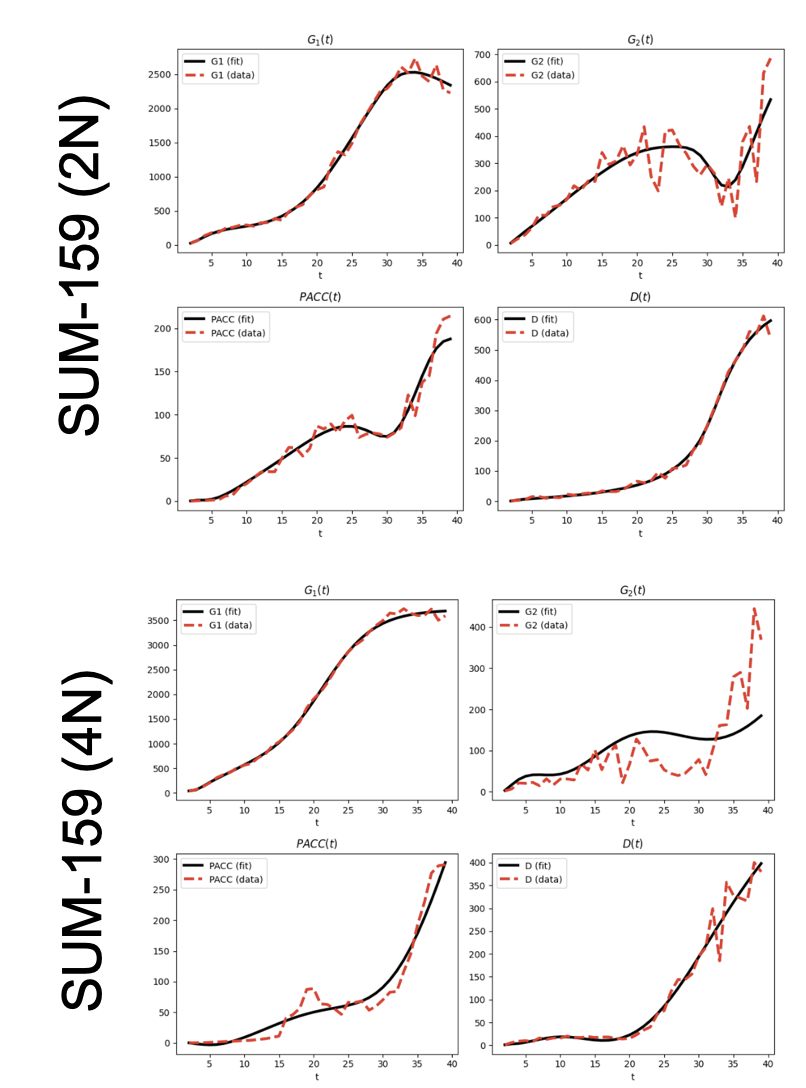
\includegraphics[width=0.9\textwidth]{Figs/ODEModelFits.png}
% \caption{\textbf{XX}.
% }
% \label{ODEModelFits}
% \end{wrapfigure}

\clearpage




\subsection{In-vivo experiments} \label{invivo}

This study utilized near-diploid (2N) and near-tetraploid (4N) variants of the SUM159 triple-negative breast cancer cell line (\texttt{SUM159\_NLS\_2N\_A6M} and \texttt{SUM159\_NLS\_4N\_A4M}, respectively). For the \textit{in vivo} experiments, 1~$\times$~10$^6$ cells were injected orthotopically into mice. A total of 40 mice were used, divided into two main groups based on the injected cell line:
\begin{itemize}
    \item \textbf{2N group:} 20 mice were injected with the near-diploid cell line.
    \item \textbf{4N group:} 20 mice were injected with the near-tetraploid cell line.
\end{itemize}
Within each group, mice were further randomized into four Gemcitabine treatment arms (n=5 mice per arm): 0~mg/kg (vehicle), 30~mg/kg, 60~mg/kg, or 120~mg/kg. Tumors were harvested at specified endpoints.

\subsection{In-vivo derived scRNA-seq analysis}

Single-cell RNA sequencing was performed on a subset of 18 tumors, including 2 metastatic lesions ans 16 primary tumors selected to include all vehicle-treated tumors and representative samples from high-dose groups exhibiting treatment failure. No tumor cells had high enough quality among the two metastatic lesions.

The two cell lines (\texttt{SUM159\_NLS\_2N\_A6M} and \texttt{SUM159\_NLS\_4N\_A4M}) were also sequenced, yielding a total of 20 scRNA-Seq datasets.


\subsubsection{Single-Cell RNA-seq Data Preprocessing and Quality Control}
Raw sequencing data was processed using the 10x Genomics Cell Ranger pipeline to generate feature-barcode matrices. As the experiment was conducted using an orthotropic mouse model, raw data was aligned to a combined human (GRCh38) and mouse (mm10) reference genome. Each cell was then classified as either human (tumor) or mouse (tumor microenvironment) based on the species to which the majority of its UMIs aligned. Only cells unambiguously assigned to one species were retained. 

For each sample, further quality control was performed independently. Low-quality cells were identified and removed based on standard metrics, including the number of unique molecular identifiers (UMIs), the number of detected genes, and the percentage of mitochondrial gene expression. Specifically, cells with an unusually low or high number of detected genes, or with a mitochondrial gene content exceeding 10\%, were excluded from downstream analysis to remove empty droplets, cellular debris, and stressed or dying cells. Following filtering, the gene expression data for each sample was normalized using the \texttt{SCTransform} method in the Seurat R package (v4), which stabilizes variance and identifies high-variance features.

\subsubsection{Copy number analysis}

\paragraph{Numbat:} Single-cell copy number profiles were inferred using Numbat. For the diploid setting, 2N tumor cells was analyzed together with a 10\% spike-in of 2N cell line cells, whereas for the tetraploid setting, 4N cells were analyzed with a 10\% spike-in of 4N cell line cells. Reads mapped to the human reference genome (GRCh38) were retrieved from 10x Genomics BAM files and used to compute phased allele counts at single-cell resolution, using haplotype information from the 1000 Genomes Project as the reference panel. Copy number states were estimated by jointly modeling allele-specific counts and gene expression matrices within the Numbat framework, using the following parameters: $t$=1e-5, $initial$ $k$=3, $min$ $genes$=10, $max$ $entropy$=0.5. Chromosome 2 was specified as the diploid reference for 2N cells, and Chromosome 13 was specified as the diploid reference for 4N cells. A diploid reference derived from the Human Cell Atlas was applied in both settings.

\paragraph{Bayesian Shrinkage Adjustment of Segmental Copy Number by Expression:}

For each genomic segment \(i\) with an a~priori copy number estimate \(c_i^{(0)}\), we refined copy number values by integrating expression data derived from matched RNA profiles. Gene-level normalized expression values were first smoothed using a 400-gene rolling mean across genomic coordinates. Each gene was then assigned to the segment(s) it overlapped, and the mean rolling expression per segment (\(e_i\)) was computed. To relate expression and copy number on a genome-wide scale, we fit a robust linear model
\[
\log(1 + e_i) = \alpha + \beta \log(1 + c_i^{(0)}) + \varepsilon_i,
\]
using Huber weighting to down-weight outlier segments (\texttt{MASS::rlm} with \(\psi = \text{psi.huber}, k=1.5\)).  
For each segment, the expression-implied copy number was obtained by inverting the fitted relationship:
\[
\hat{c}^{\text{expr}}_i = \exp\left(\frac{\log(1 + e_i) - \alpha}{\beta}\right) - 1.
\]
Uncertainty of this estimate was approximated using the delta method,
\[
\sigma_{\text{expr},i}^2 \approx \left[\frac{1}{\beta}(1 + \hat{c}^{\text{expr}}_i)\right]^2 \sigma_\varepsilon^2,
\]
where \(\sigma_\varepsilon^2\) is the residual variance of the regression.  
An empirical prior variance \(\sigma_c^2\) was computed from the deviation between prior and expression-implied copy numbers, \( \sigma_c^2 = \mathrm{Var}(c_i^{(0)} - \hat{c}^{\text{expr}}_i) \).  
For each segment, the maximum a~posteriori (MAP) adjusted copy number was then obtained by Bayesian shrinkage toward the prior:
\[
\hat{c}^{\text{MAP}}_i = \frac{\sigma_{\text{expr},i}^{-2} \hat{c}^{\text{expr}}_i + \sigma_c^{-2} c_i^{(0)}}{\sigma_{\text{expr},i}^{-2} + \sigma_c^{-2}}.
\]
This formulation balances expression-derived evidence against the genomic prior according to their respective uncertainties.  
To prevent biologically implausible values, adjusted copy numbers were truncated to the range \([1,6]\).  
The procedure returns both the fitted regression parameters (\(\alpha, \beta, \sigma_\varepsilon^2, \sigma_c^2\)) and a per-segment table containing prior, expression-implied, and MAP-adjusted copy numbers for downstream analysis.

XX: we did the same for 2N and 4N cells, I do not think it works so well in 2N cells because sequencing saturation is lower. need to include Xiaoqing's saturation analysis



\clearpage




\subsubsection{Integration of scRNA-seq Datasets}
To create a unified dataset and correct for technical batch effects arising from separate sequencing runs and experimental conditions (2N vs. 4N tumors; variable Gemcitabine doses), the normalized data from all samples were integrated. We employed the Canonical Correlation Analysis (CCA) integration workflow within the Seurat v4 toolkit. This method identifies shared sources of variation between datasets, or ``anchors,'' which are then used to harmonize the datasets into a single, integrated analytical object. The integration allows for direct comparison of cells across all experimental conditions by minimizing technical variability while preserving biological differences.


\subsubsection{Unsupervised Clustering and Dimensionality Reduction}
After integration, we performed dimensionality reduction on the combined dataset to identify the major axes of variation in the data. Principal component analysis (PCA) was conducted on the integrated gene expression matrix. The top 30 principal components (PCs), which captured the majority of the biological variance, were selected for downstream analysis. These PCs were then used to construct a shared nearest neighbor (SNN) graph, which identifies cells with similar transcriptional profiles. The Louvain algorithm was subsequently applied to the SNN graph to partition the cells into unsupervised clusters. For visualization and exploration of the cellular landscape, Uniform Manifold Approximation and Projection (UMAP) was run on the selected PCs to generate a two-dimensional embedding of the single-cell data.

\subsubsection{Cell Type Annotation and Cell Cycle Scoring}
The unsupervised clusters were first separated into human (tumor) and mouse (tumor microenvironment, TME) populations based on their species of origin. To identify specific cell types within the TME, the mouse cell clusters were analyzed for the expression of canonical marker genes. For example, immune cell populations such as neutrophils, T-cells, and macrophages were identified by their expression of established lineage markers.

To investigate proliferative states, cell cycle phase was computationally inferred for all cells (both human and mouse). Using the \texttt{CellCycleScoring} function in Seurat, cells were assigned scores based on their expression of G2/M and S phase-specific gene sets. Each cell was then assigned a phase (G1, S, or G2/M), providing a quantitative measure of cell cycle activity across all experimental conditions.


\subsubsection{Differential Expression and Pathway Analysis in Tumor Cells}
To identify transcriptional programs associated with Gemcitabine treatment and ploidy, differential gene expression (DGE) analysis was performed on the human tumor cell population. We used the Wilcoxon Rank-Sum test implemented in the Seurat \texttt{FindMarkers} function to compare gene expression between dose conditions (e.g., 120~mg/kg vs. vehicle) within each ploidy lineage (2N and 4N) separately. Genes were considered significantly differentially expressed with an adjusted p-value of $<$ 0.05 after Bonferroni correction.

To assess specific biological states, we scored each cell for the expression of curated gene sets related to chromosomal instability (CIN) and hypoxia using the \texttt{AddModuleScore} function. These scores were then compared across ploidy and dose groups. Broader pathway-level changes were assessed using Gene Set Enrichment Analysis (GSEA) on the ranked list of differentially expressed genes to identify enrichment of pathways from the MSigDB Hallmark collection. Finally, to find pathways directly correlated with ploidy, we fit linear models between continuous ploidy values and pathway module scores \color{blue} within and across 2N- and 4N- groups \color{black}.

\subsubsection{Analysis of the Tumor Microenvironment (TME)}
To investigate how tumor ploidy shapes the TME, we focused on the mouse cell population. First, we performed a compositional analysis by calculating the relative proportion of each annotated TME cell type (e.g., neutrophils, T-cells) within 2N-derived versus 4N-derived tumors. The significance of changes in cell proportions was assessed using a chi-squared test. 

Second, to identify functional differences in TME components, we performed DGE analysis specifically on the neutrophil population, comparing cells isolated from 2N tumors to those from 4N tumors. This analysis, using the Wilcoxon Rank-Sum test, aimed to reveal differences in the transcriptional state of neutrophils that are sculpted by the ploidy of the surrounding tumor.

\subsubsection{Modeling Cell Cycle Activity}
To test the hypothesis that Gemcitabine dose and tumor ploidy collectively predict cell cycle activity, we utilized the cell cycle phase assignments (G1, S, G2/M) for the human tumor cells. We fit a multinomial logistic regression model, which is appropriate for a categorical outcome with more than two levels. \color{blue} The model was specified as \texttt{CellCyclePhase \textasciitilde{} Ploidy\_Group + Gem\_Dose}, where \texttt{Ploidy\_Group} was a continuous variable quantified from each tumor's karyotype (Section XX) and \texttt{Gem\_Dose} was also a continuous variable. The significance of the coefficients for each predictor was evaluated (p $<$ 0.05) to determine if dose and ploidy are significant predictors of the probability of a cell being in a given phase of the cell cycle. The same analysis was repeated using tumor diameter as outcome variable instead of cell cycle state.\color{black}







\end{document}